\chapter{Research Methodology}
%\chapter{Research methodology}
\section{Data and tools}
World wide non governmental organizations publish some of their reports on their official websites.  Web scrapping is one of the ways to extract data from website to the local machines. We downloaded the reports about appeals in pdf format from IFRC website. 
We used R-scripts for web scraping form our co-supervisor  Xavier Vollenweider 
%\Jnote{Is Xavier formally co-supervisor? If yes, you should put him on the
%  front page. Is he a professor? Please clarify this. Also use his full name.}
 
We downloaded 1262 reports which have been submitted between $ 1^{st}$ January 2015 and $31^{st}$ December 2016. To differentiate the reports, each report has  a report Id but different reports can refer to the same appeal Id. Appeal Id is a unique number given to a  specific disease.
%\Jnote{What is appeal id? Please explain.}
As an international organization which works
%\Jnote{``Which insights''? I don't understand what you mean here.}
on the largest humanitarian  activities in the world,
IFRC reports we have talk about disasters and cash transfer program.
Cash Transfer Program (CTP) describes the money used by IFRC to buy food, shelter, etc. For example the mon
%\Jnote{Try describing better what CTP is.}
%\section{Data Analysis and Filtering}
\section{Supervised vs Unsupervised  Machine Learning}
\begin{itemize}
\item \textbf{Supervised} is a machine learning part which deals with "labelled data",  data are categorized and classified.

 We have a csv document which summarizes
the appeals that we have. The shape of this document is 25 columns and 3997 rows. The "CTP" feature indicate if the appeal is classified as a Cash
  Transfer Program document  or not. Among 3997 appeals, 404 are CTP.
%  \Jnote{Please explain how the CSV file relates to your data.}
  %\Jnote{Make two paragrahps: one with definition of SL and one introducing
  %  your example.}

\item \textbf{Unsupervised} can be defined as a way machine learning processes ”unlabelled data”.
the data are unstructured, uncategorised and unclassified. The reports we have are good example of unlabelled data.
\begin{itemize}
\item Clustering is a technique for analysing data by identifying hidden groups in a data set. The hidden groups helps the machine to  classify them data into small groups called "cluster" based on similarities or relationship found in data \citep{dy2004feature}.
\end{itemize}
\section{NLP Corpus Preprocessing }\label{re}

Portable document format (PDF) has content which can not be extracted and manipulated  easily. Our data have to be changed into another format in order to pull the information we need. We managed to transform 1260 reports.  Our folder has 1260 transformed reports

files which is considered as dataset. For analysing the data, we used  Python programming language.

Our data reported on different areas of the World such as continents, countries and cities. For example "Europe IB23102015 23Oct2015.txt" covers European continent , "Afghanistan MDRAF003 05Nov2015.txt" and  "Japan 0 16Apr2016.txt" reported  on specific countries and  "Port au Prince country cluster 0 04Oct2016.txt" reported on the most populous city of Haiti.


Corpus is a set of large data which are semi-structured.  To extract entities from corpus is simpler than to deal with unstructured data. To get the corpus we filtered the data by using unicode of utf-8 and removing non-printable characters.

To get compatible data, we have to filter using the Unicode provides canonical and compatible equivalence.


\textbf{Regular Expressions} are for searching matched patterns in string.  
in Python, regular expression has operations and modules like "re.py" aND so on. they are used to manipulate characters in strings. regular expressions use a backslash $(" \backslash  ")$  to indicate a special form without invoking the meaning of the special form. There are many regular expressions functions but some of what we used the most are :
\begin{itemize}
\item re.split(): this function split pattern and return the list of string.
\item re.search(): it returns matching  objects.
\item the match object ".end()": in a search string, it returns the end position of the match.
\item the match object: in a search string, it returns the start position of the match.
\end{itemize}

\textbf{ASCII} stands for American Standard Code for Information Interchange. it is uses numbers to represent text by using 128 characters. Computer uses ASCII exist within unicode for storing texts easily. All  ASCII uses unicode.

ASCII characters are used to send and receive the e-mails, for text files and data conversions. 

\begin{figure}[hbtp]
\caption{ASCII TABLE \citep{witte2002electronic}}
\centering
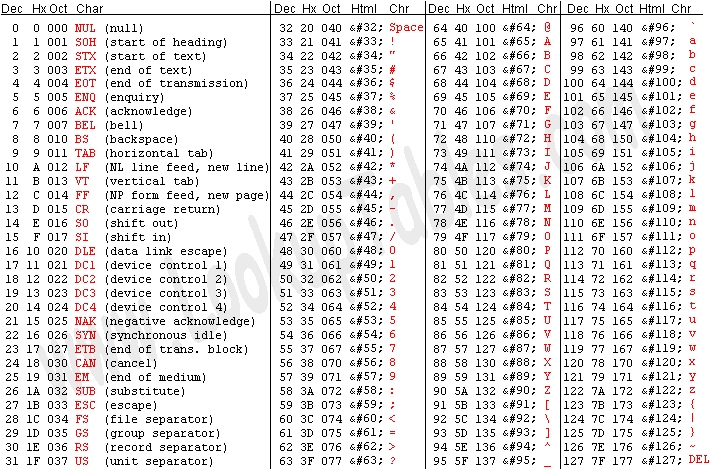
\includegraphics[scale=.35]{images/ASCII.png}\label{ASCII}
\end{figure}
\end{itemize}
%\end{itemize}

Figure \ref{ASCII} demonstrates Unicode  standard.
It provides  a unique number to each character composing a text regardless the language, program  or platform.

UTF stands for Unicode Transformation Format. Due to the fact that unicode can't fit into one 8-bit bytes, there are many  different types of UTF which store unicode in byte of sequence.  characters are set into binary values 0 and 1. UTF-8 for encoding  8 bytes, UTF-16 for encoding 16 bytes and UTF-32 which is a standard for encoding 32-bytes are three current standards. For our corpus we used UTF-8.

After getting semi-structured documents, we removed the stop-words

which are defined as unnecessary words for extraction of entities from corpus.

Normally the stop-words return vast amount of unwanted information. Some example of English Stop Words: almost, are, or,  details, during, upon and so on.

Now we can check how for all of 1260 documents and count the Stop Words to be removed from vocabularies of corpus. We trained corpus by nltk package called FreqDist which uses  frequency distribution of each word occurs in corpus, then the module of nltk technique called "nltk.corpus.PlaintextCorpusReader" helped us to get total 58104 stop words over the whole  7796263  vocabularies.

\section{Modules and packages}
The procedure of extracting entities requires many linguistic packages. Machine learning algorithms check grammar rules, punctuation marks and syntaxes. Some
documents can have special characters such as emoticons for emotions. To choose the packages to use, it is recommended to understand clearly how they work and the content type of your documents. This is a list of packages we used for extracting IFRC entities.
\begin{itemize}
\item \textbf{os} : This module is  known as miscellaneous operating system interfaces. os represents the functionality of operating system with independent functions such as os.path.isfile(), os.path.exist, os.path.isdir, etc.  

  Its functions are important for building platform-independent programs. The programs written  using os module  can execute in Windows and Linux regardless the machine operating system. 

\item \textbf{nltk}: Natural Language Toolkit is one of core packages for linguistic modelling . With various important  built-in functions nltk is able to manipulate documents.  The main idea behind nltk is to use $nltk_{-}corpus$ to collect all documents as one dataset, then split the documents into sentences using $ne_{-}chunk$ and  remove the stop-words by  importing $stopword$ from $ntk.corpus$, lastly apply machine learning algorithms to extract entities.

\item \textbf{PyPDF2} is able to extract specific information from a pdf document based on the section they belong to. This package locates top section, title, author, etc. It has many functions such as splitting documents pages, merge document pages, encrypt and decrypt documents and so on. It can be compared to pdftk
\item \textbf{pandas} is an open source with high performance structure within various build in functions.
  Dataframe design for presenting many data in organized way. Pandas is powerfull in data analysis, flexible, fast and manipulation took for any language. In our research, We used pandas for making the frames of our data.
  
\item \textbf{codecs} module  offers unicode string for encoding and decoding. codecs is used for handling errors and gives freedom to access internal registry. Codecs are not limited to text but mostly are for text encodings which is for encoding text to bytes. Additionally, there exits codecs for encoding text to text, some codecs can encode and decode at the same time.
\item  \textbf{defaultdictionary} has basic content of difference between verbs, nouns, adjectives, adverbs etc.  Defaultdict in Python  a dictionary with default value for missing key instead of key error.

\item \textbf{Python String Strip} is a module which has methods to  returns a string with trailing text removed. Two methods to strip text on both sides, rstrip for right hand side and lstrip for left hand side. Trailling text can be  unwanted space, extension, punctuation marks, etc.

To indicate the position of the character to be stripped we use left(l.strip()) which removes the character at the beginning of a string or right(r.strip()) to remove the character at the end of the string.
\item \textbf{regular expressions } regex is a module which finds out the patterns between strings by setting rules for text. bytecodes compile those pattern rules and execute using matching rules.  example methods for re are explained into Chapter \ref{re}
\item \textbf{polyglot} is used to extract entities from many languages.  It is multilanguage application supporter built as natular language pepeline.
\item \textbf{Stanford} is one of most brilliant algorithms to extract entities from  documents corpus. it has classifier models, jar files which are free downloads. Stanford has many packages to handle linguistic problems. 
\end{itemize}

\section{Extraction of Entities }

To extract entities we used default dictionary built in collection package of nltk. Our dataset now is a folder containing 1260 corpus files, we  used nltk chruncker to get sets of lines  from our corpus. let have a look for our sample document the way lines are split.
\begin{figure}[hbtp]
\caption{Set of sentences}
\centering
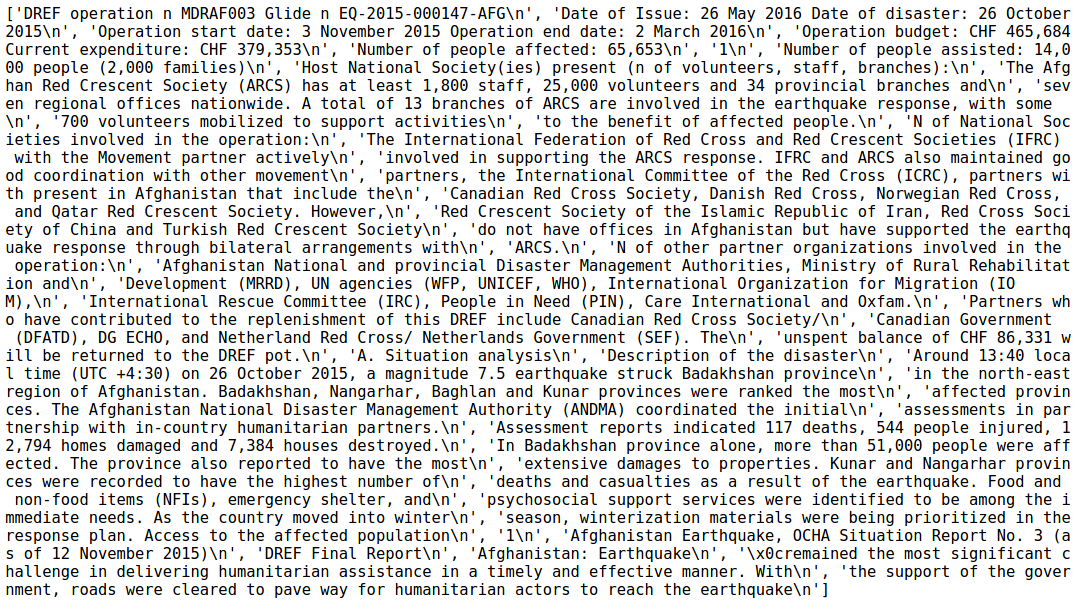
\includegraphics[scale=0.4]{images/corpus.png}\label{Set of sentences}
\end{figure}


Figure \ref{Set of sentences} shows the 45 first lines of the sample document. each each line is ended by  $'\backslash n'$.

\section{Top Section Dataset \label{top}}

From the analysis of IFRC pdf reports, most of them have a small table on the top. this table gives the image of what the report is talking about. This table summarizes what the document is talking about. For example the total amount of money spent in recovering a disease, the number of people who participated in a given activity, the location and so on.

While we were transforming the pdf data into txt format, this table occupied almost 25 first lines. Due to the limited time of the research, We decided to split those twenty five first lines of each document. the collection of those first twenty five documents has been considered as our new corpus.

Now  we can use  one of the algorithms to extract entities and for classification.
\section{Stanford Named Entities Recognition}

The data to be trained is unlabelled. Named Entities Recognizer labels the data to be extracted easily. it recognises sequence of words and its classification is mainly to name of persons, localization and organization.

Stanford Named Entities Recognition is an extractor implemented in java. It takes the sequence of words and label them 
Stanford named entities recognition is  a able to identify correctly the named recogniser which labels sequences of words in a text. The next step is to split the sentences into set of words called tokens. By using the Stanford NER tokenizer  where token can be tagged. 

\begin{itemize} 
\item \textbf{Stanford NER Tagger} is a package which has modules for classifying tokens with the taggs. A tagg can be defined as one of classes of significant words like nouns, adjectives etc. we used the package Stanford POS Tagger to classify the words. 
\item \textbf{Stanford NER Models} are many Stanford has different models such as "stanford-corenlp-full-2016-10-31", "stanford-ner-2014-01-04" which is the version we used. 

\item \textbf{Stanford Classifier} is a package which classify the entities into defined categories. It has four specific classes such as  "Locations",  "Persons",  "Organizations" and    "Others".
\end{itemize}

We specified the named entities that we wanted to extract. We classified them into the four categories by Stanford classifier.  The last category called "others" combined all numerical entities such as time, amount of money, number of people, percentage, etc. 

The reports from our corps are order by appeal numbers, the entities are in classified by Stanford algorithm. 

\begin{figure}[hbtp]
\caption{IFRC entities from Stanford NER}
\centering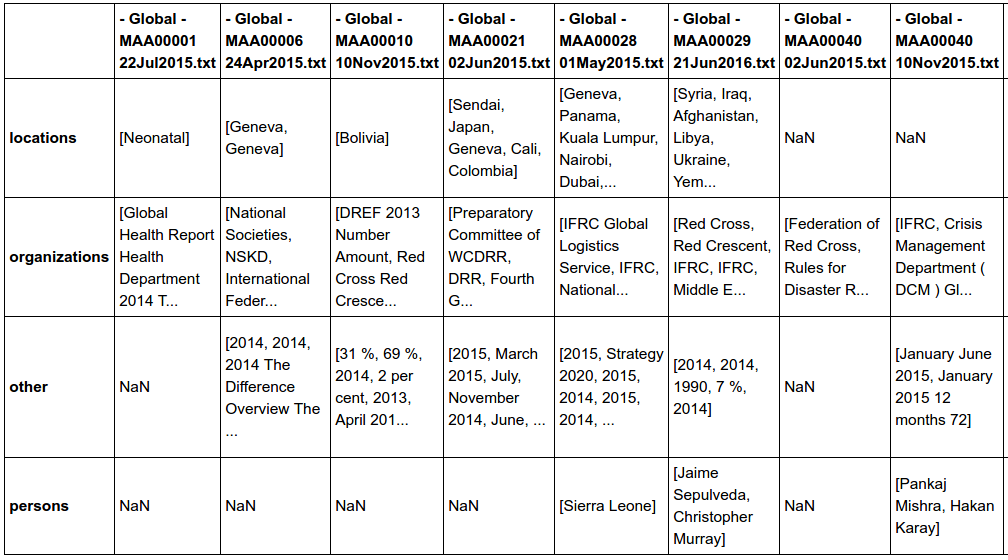
\includegraphics[scale =.45]{images/stanford.png} \label{stanford}
\end{figure}
From Figure \ref{stanford},  Consider the for the report "-Global MAA00029 21Jun2016.txt", locations row  shows that the report covered Syria, Irak, Afganistan, Libia, Ukraine, Yemen, etc.
The extraction of entities separates clearly the categories.
\section{Natural Language ToolKit (NLTK)}
Natural Language ToolKit is one of the algorithm to extract named  entities. It has different modules which are used to process the data alongside the extraction.
NLTK chunkparser is a one of nltk module  which uses Regular expressions. NLTK tokenize which splits the sentences into small units called tokens. This module helps the NLTK tagger to identify words independently. 

Generally NLTK classify the entities into four categories which are known as Locations, Organizations, Persons and Others.

\begin{figure}[hbtp]
\caption{IFRC entities from NLTK}
\centering
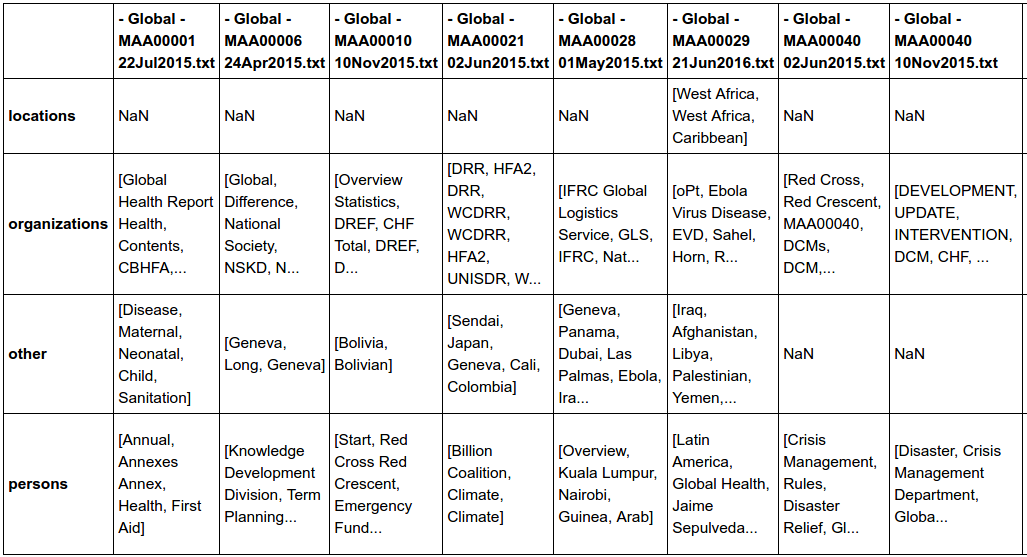
\includegraphics[scale=.45]{images/nltkalgo.png}\label{nltkalgo}
\end{figure}

From Figure \ref{nltkalgo}, Consider organizations extracted from the report "-Global-MAA00021 02 Jun 2015.txt", NLTK entities classifier was able to extract DRR, HFAR, WCDRR, HFAR2, UNISDR, etc. The classifier uses nltk tagger and default dictionary which help it to identify the names, verbs and adjectives.

For NLTK algorithms, some confusion between two categories "Location" and "Others" which might be fixed later.

\section{Polyglot Named classifier}

Compared to previous entities extractor, Polyglot has only three categories which are "Persons", "Locations" and "Organizations". For nltk, any entity which is not classified into those three categories is not considered as named entity.
\newpage

\begin{figure}[hbtp]
\caption{IFRC entities from Polyglot}
\centering
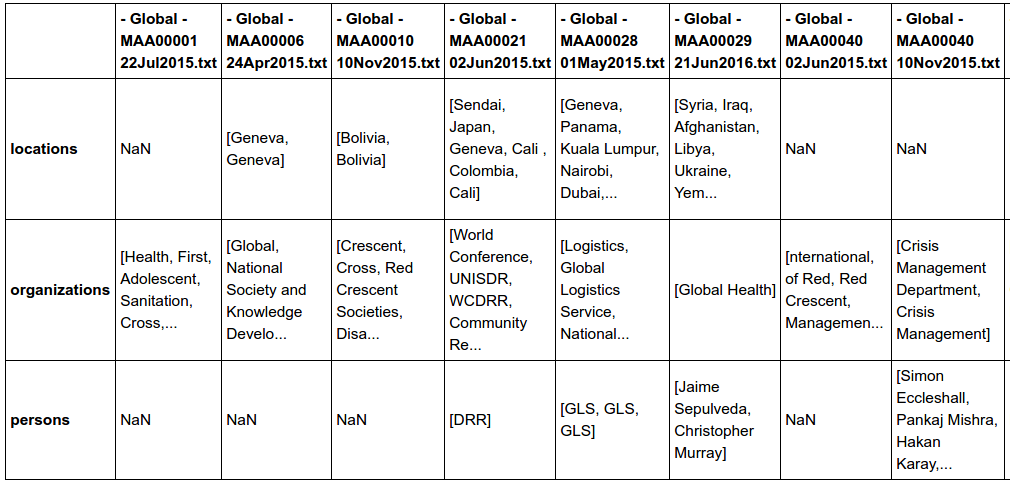
\includegraphics[scale=.5]{images/polyglot.png}\label{polyglot}
\end{figure}
Let us take an example report "-Global-MAA000029 21 Jun 2016.txt" from Figure \ref{polyglot}, the entities which are classified as "Persons" Jaime, Sepulveda and  Christoper Murray.




%\section{Sample Files} 
%The type of data we have can be considered into two different ways. There are some reports which are classified as CTP documents. This documents cover the overview of how IFRC money was invested in humanitarian activities.
%
%Non CTP reports are focused on other activities which didnt require IFRC to invest money. 
%
%The next step is to take example report document for CTP and Non-CTP to have a comparison on the extracted entities.  
%































%\section{Entities Recognition and Classification}
%%\newpage
%\begin{figure}
%        \begin{subfigure}{0.5\textwidth}
%         \caption{Organizations sample}
%                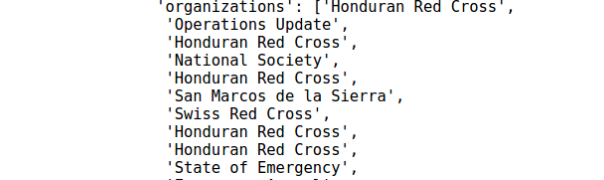
\includegraphics[width=\textwidth]{images/organizations.png}
%                \label{Organizations}
%        \end{subfigure}%
%        \begin{subfigure}{0.5\textwidth}
%        \caption{Location sample}
%                
\includegraphics[width=\textwidth]{images/location.png}
%                \label{Location}
%        \end{subfigure}\\
%        \begin{subfigure}{0.5\textwidth}
%         \caption{Person's names}
%                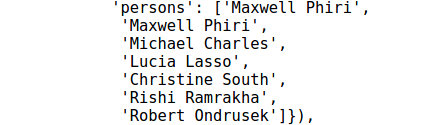
\includegraphics[width=\textwidth]{images/person.png}
%                \label{Persons}
%        \end{subfigure}%
%        \begin{subfigure}{0.5\textwidth}
%        \caption{Others category}
%                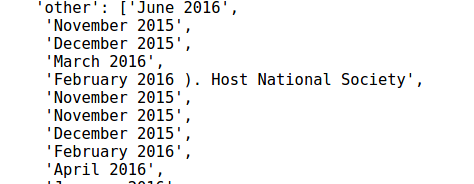
\includegraphics[width=\textwidth]{images/others.png}
%                \label{Others}
%        \end{subfigure}
%\end{figure}
%
%\section{Entities linking}
%Natural languages used by human are inherently noisy, spelling mistakes and ungrammatical mistakes. Machine learning algorithms are able to handle linguistic problems.  
%\section{Context}
%\section{Bag of words}

%
%
%The frequency of a word is calculated based on summation of times the word appeared into a document. The frequency is used in words classifiers.
%
%\section{Mathematics behind entities extraction}
%\section{Supervised Classification}
%They are key points to classify the data which are supervised:
%
%\section{Corpus from Natural Languague Tolkit}

%The check-up on the entities extracted from the text can be done by comparing what has been extracted by hands and what the algorithm give us as results.

%The check-up on the entities extracted from the text can be done by comparing what has been extracted by hands and what the algorithm give us as results.
